\chapter{Technische Grundlagen}

Da die Erkennung, Lokalisierung und Handhabung der Objekte eine Interaktionsfähigkeit zwischen dem verwendeten Kamerasystem, einem Objekterkennungsalgorithmus und der Robotersteuerung voraussetzen, werden in diesem Kapitel notwendige Grundlagen und für die Umsetzung angewandte Techniken erläutert.

%\section{Industrieroboter} \ver
%Mit der stetigen Weiterentwicklung der Industrie werden die Aufgabenbereiche immer komplexer und nehmen viel Zeit in Anspruch. Um den Menschen von dieser schweren Arbeit zu entlasten und die Produktivität zu steigern, werden heutzutage Industrieroboter in nahezu jedem Bereich verwendet. Die enorme Belastbarkeit sowie Flexibilität der Roboter macht diese zu optimalen Arbeitsmaschinen. Bei Industrierobotern gibt es wesentliche Unterschiede in der Bauweise und in der Softwaresteuerung. Dabei kann zwischen mobilen und stationären Robotern unterschieden werden (\refFig{fig:Einteilung_Roboter}).

%\begin{figure}[ht]
%    \centering
%    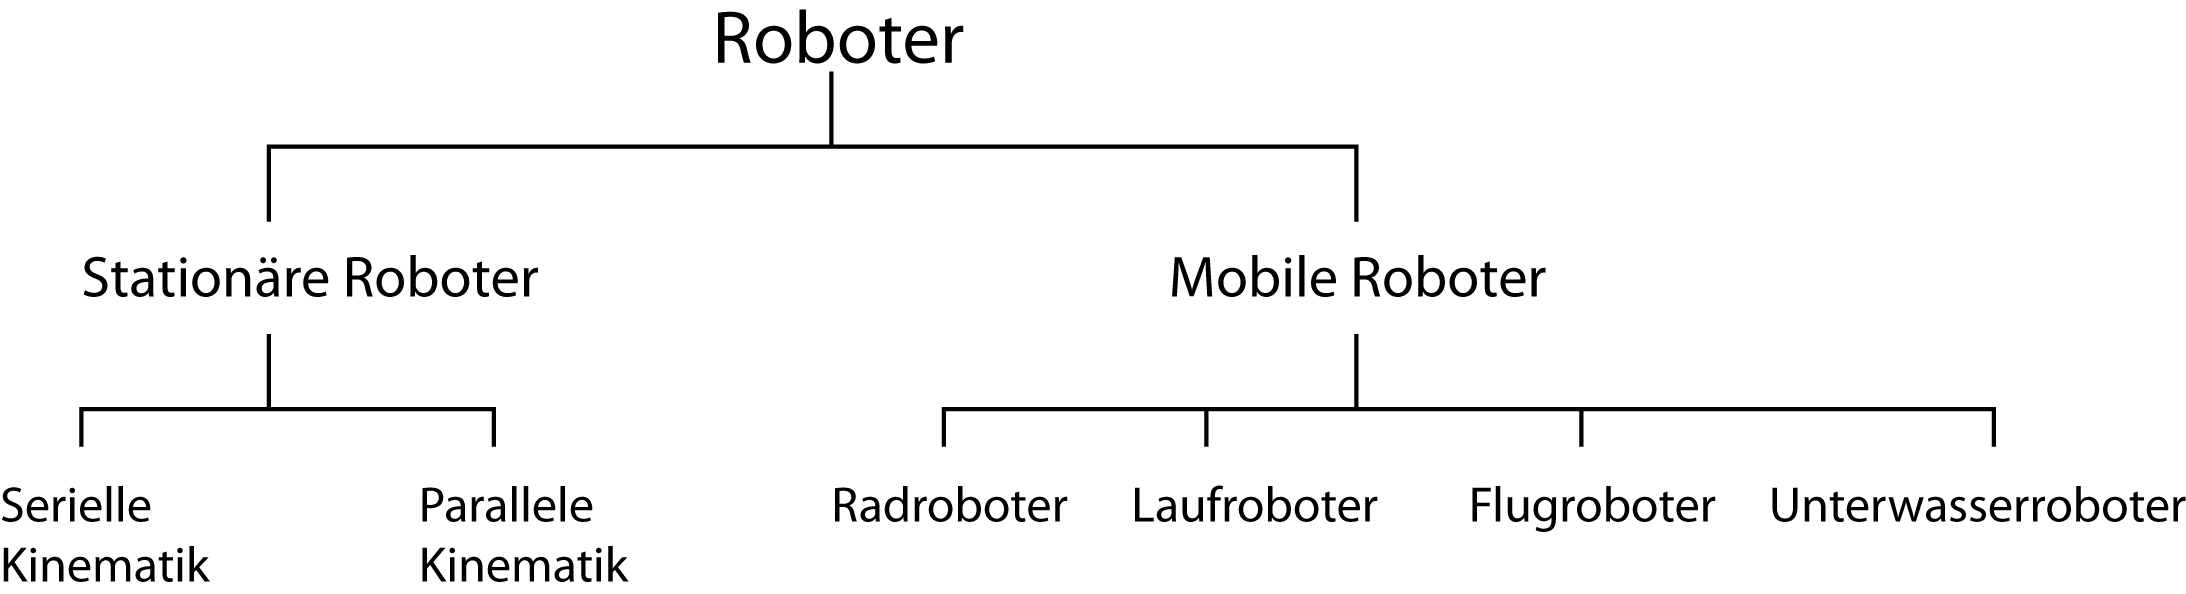
\includegraphics[width=\textwidth]{Bilder/Industrieroboter_unterteilung.png}
%    \caption{Einteilung Roboter \cite[Abbildung~1.1]{wust_grundlagen_2018}}\label{fig:Einteilung_Roboter}
%\end{figure}

%Die Anforderungen an die Automatisierung von Industrierobotern steigen stark. Deshalb ist es notwendig die Robotersteuerungen weiterzuentwickeln, um immer mehr Möglichkeiten zu bieten. Alternativ gibt es auch die Möglichkeit einer modernen Schnittstelle zu bestehender Hardware. Im Folgenden werden die aktuellen Systeme näher erörtert.

%\subsection{Steuerungssoftware} \ver
%Üblicherweise werden Industrieroboter mit der jeweiligen Herstellersoftware angeboten. Die Softwaresteuerung ist bereits auf das Produkt abgestimmt, was dazu führt, dass die Roboter nur schwer mit einer anderen Software verwendbar sind. Dementsprechend ist dieser an einen Hersteller gebunden und ist je nach Anwendung in der Funktionalität eingeschränkt. Der Vorteil liegt darin, dass auftretende Probleme vom Hersteller direkt schnell behoben werden können und die Funktionalität des Industrieroboters in Verbindung mit der Software optimiert wird.

%Um dem Kompatibilitätsproblem zu entgehen, kann man eine Open-Source-Software namens \ac{ROS} Industrial verwenden. Genauer wird dies in \ref{sec:Robot_Operating_System} erläutert. Es gibt nur wenige Open-Source Alternativen zu \ac{ROS}, die lediglich spezielle Anwendungsbereiche abdecken.

%\subsection{Bahnsteuerung} \ver
%Die Ansteuerung eines Punkts im Raum kann auf mehrere Weisen an die Robotersteuerung übergeben werden. Dabei unterscheidet sich die Art der Bewegung des \ac{TCP}. Die zwei folgenden Bahnsteuerungsarten sind die wesentlichen Steuerungsmöglichkeiten für einen Roboterarm, aber hier handelt es sich lediglich um die Grundfunktion, die mit weiteren Methoden verfeinert werden können.
%\begin{description}
%    \item[Point to Point] \textit{\ac{PTP}} ist eine Art der Bewegungsprogrammierung eines Roboterarms, die mit der direkten Verbindung zwischen Start- und Zielkoordinate arbeitet. Man unterscheidet zwischen einer Asynchronen- und Synchronen-\ac{PTP}-Steuerung. Letztere hat den Vorteil, dass die Bewegungen der Achsen gleichzeitig starten und stoppen. Das führt zu einer geringeren Bahnabweichung des \ac{TCP}, dennoch kann die Bahn des Effektors stark von der direkten Verbindungslinie des Start- und Zielpunkts abweichen. Deshalb ist diese Methode nicht für eine Bahnführung mit hohen Genauigkeitsanforderungen geeignet. Der Vorteil liegt in der schnellen und einfachen Bewegungsplanung.

%    \item[Continuous Path] Eine \ac{CP}-Steuerung, auch kartesische Bahnsteuerung genannt, ist eine Methode zur exakten Einhaltung der geforderten Bahn des \ac{TCP}. Dabei werden zwischen Start- und Zielkoordinate sogenannte Interpolationspunkte (Zwischenpositionen) berechnet, denen der Roboterarm folgen soll. Hierfür muss jedoch die passende Roboterstellung in Form von Gelenkwinkeln für jeden Punkt gefunden werden, damit eine gleichmäßige Bewegung des Arms entsteht. Diese Methode eignet sich besonders gut für Aufgaben mit einer hohen Präzisionsanforderung.

%\begin{figure}[ht]
%    \centering
%    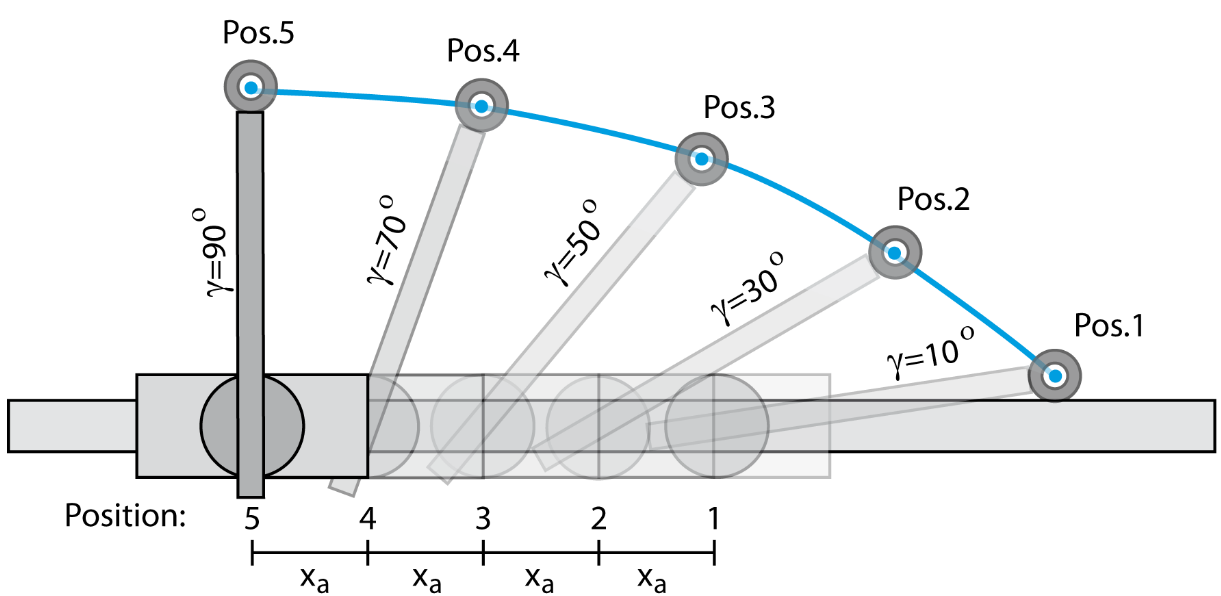
\includegraphics[width=\textwidth]{Bilder/Point_to_Point.png}
%    \caption{\ac{PTP}-Steuerung mit Bahnabweichung \cite[Abbildung~4.3]{wust_grundlagen_2018}}\label{fig:PTP_Steuerung}
%\end{figure} 

%\begin{figure}[ht]
%    \centering
%    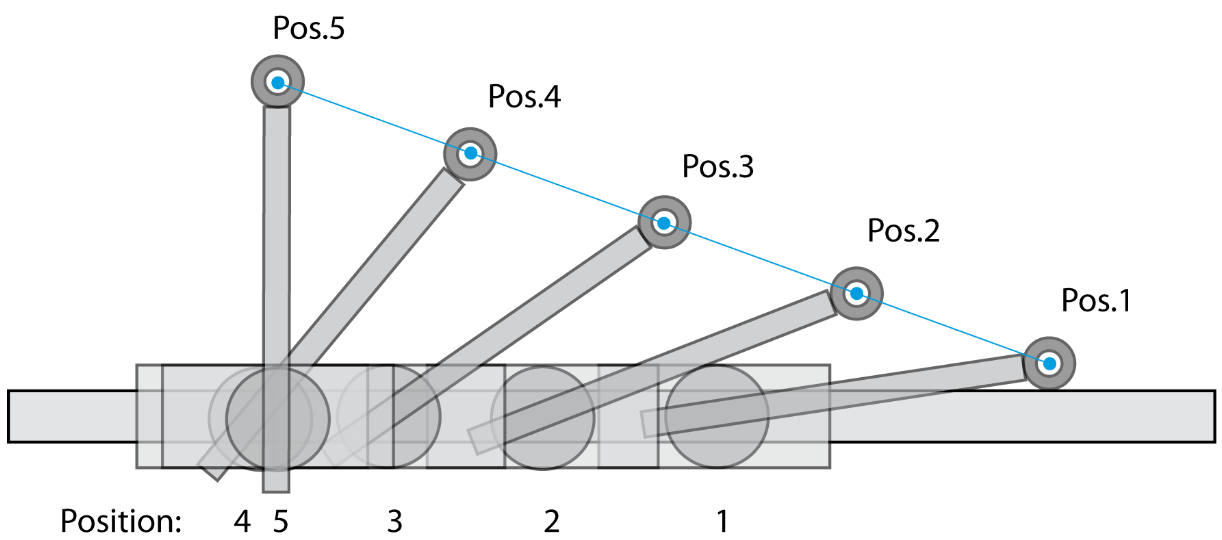
\includegraphics[width=\textwidth]{Bilder/Continuous_Path.png}
%    \caption{\ac{CP}-Steuerung ohne Bahnabweichung \cite[Abbildung~4.4]{wust_grundlagen_2018}}\label{fig:CP_Steuerung}
%\end{figure}
%\end{description} \cite{wust_grundlagen_2018}

\section{Robot Operating System (ROS)} \label{sec:Robot_Operating_System}

Die Kommunikation zwischen in der Robotik eingesetzter Hardware bereitete in der Vergangenheit aufgrund nicht vorhandener Standards bei der Datenübermittlung oft Probleme, die nur mit hohem Entwicklungsaufwand gelöst werden konnten \cite[Kapitel~1]{quigley_ros_2009}. Daher ist ein einheitliches System, das verschiedene Programme und Hardware verbindet, notwendig. Diese Problematik kann durch die Verwendung des \ac{ROS} gelöst werden. Dieses bildet mit einer Vielzahl verfügbarer Pakete eine Grundlage für komplexe Steuerungen. Es kann auf einem einzelnen Computer oder einem Netzwerk aus Computern genutzt werden und vereinfacht die Interoperabilität verschiedener Steuerungshardware. \ac{ROS} dient außerdem als Middleware, die die Kommunikation zwischen Teilen von Software ermöglicht. Die Pakete sind dabei entweder direkt auf \ac{ROS} ausgelegt, oder bilden eine Schnittstelle zu \ac{ROS} für Hardwarekomponenten oder inkompatible Software. Die Website \textit{ros.org} beschreibt das System als ein Paket aus Software und Softwarebibliotheken, mit dem Roboterprogramme entwickelt werden können \cite{rosorg_roshome_2021}.

\ac{ROS} wurde 2007 unter dem Namen \textit{Switchyard} von Morgan Quigley gestartet \cite[Kapitel~1]{joseph_mastering_2018}. Das öffentlich verfügbare \textit{Repository} wurde im Januar 2012 publiziert. Es existieren heute mehrere Konsortien für verschiedene Regionen, darunter beispielsweise das vom Fraunhofer-Institut für Produktionstechnik und Automatisierung geleitete \textit{ROS-I Consortium Europe}. Diese stellen technische Unterstützung und Training für \ac{ROS} bereit und legen Entwicklungsziele fest \cite{rosindustrialorg_brief_nodate}.
Ein großer Vorteil des \ac{ROS} verglichen mit anderen Systemen neben der Hardwareunabhänigkeit ist, dass es ein Open-Source-Projekt ist. Somit kann es gut auf alle Anforderungen angepasst werden und es kann eine Vielzahl an Programmen, die mit \ac{ROS} kompatibel sind, genutzt werden. Dabei ist laut \textit{ros.org} das primäre Ziel des Projekts nicht die Bereitstellung besonders vieler Features, sondern die Unterstützung der Wiederverwendung von Quellcode in der Forschung und Entwicklung \cite[Absatz~2]{dattalo_rosintroduction_2018}.

Nachfolgend werden der Aufbau und die Versionen des \ac{ROS} sowie Möglichkeiten zur Integration einer Objekterkennung beschrieben. Der Fokus liegt auf der im Projekt verwendeten Version ROS-I.

\subsection{Aufbau}

Anders als der Name \ac{ROS} impliziert, handelt es sich technisch gesehen nicht um ein klassisches Betriebssystem, sondern Softwarepakete, die auf bestehenden Betriebssystemen installiert werden können. Das Programm unterstützt offiziell die Linux-Distributionen \textit{Ubuntu} und \textit{Debian}, während für \textit{Windows} und \textit{Arch Linux} experimentelle Versionen zur Verfügung stehen \cite{wikirosorg_noeticinstallation_2020}. Die empfohlene Installationsmethode besteht im Hinzufügen eines Repositorys, wodurch \ac{ROS} über den Paketmanager der verwendeten Linux-Distribution installiert werden kann. Gründe für die Bezeichnung als Operating System sind die Bereitstellung von Services wie Hardware Abstraktion, Paketmanagement sowie eine Kommunikation zwischen Prozessen, wobei es sich um typische Eigenschaften von Betriebssystemen handelt \cite[Absatz~1]{dattalo_rosintroduction_2018}.

\ac{ROS} ist grundsätzlich in mehrere Teile gegliedert. Die offizielle Dokumentation unterscheidet hier zwischen dem ,,Filesystem Level'', ,,Computation Graph Level'' und ,,Community Level'' \cite{romero_rosconcepts_2014}. Für eine bessere Übersicht wird hier zwischen \textbf{Paketmanagement}, \textbf{Struktur} und \textbf{Entwicklung und Dokumentation} unterschieden und verstärkt auf die für diese Arbeit relevanten Teile eingegangen.

\subsubsection{Paketmanagement}

Das Paketmanagement des \ac{ROS} kann in folgende Punkte gegliedert werden:

\begin{description}
    \item[Packages] \textit{Packages} bilden die Grundlage für die Organisation von Softwarekomponenten. Die Softwarepakete enthalten alle notwendigen Teile eines einzelnen Programms. Eine spezielle Art von Packages sind Metapackages, bei denen es sich um eine Zusammenstellung mehrerer Einzelpakete handelt \cite[Absatz~1]{romero_rosconcepts_2014}.
    \item[Repositories] \textit{Repositories} sind Paketquellen, die ein oder mehrere Softwarepakete zum Download bereitstellen. Neben dem primären ROS-\textit{Repository}, das essenzielle Pakete enthält, können Institutionen oder einzelne Entwickler eigene \textit{Repositories} zur Verfügung stellen \cite[Absatz~1/3]{romero_rosconcepts_2014}.
    \item[Dependencies] \textit{Dependencies} sind \textit{Packages}, die von anderen Softwarepaketen zur korrekten Funktionsweise benötigt werden \cite[Absatz~1]{romero_rosconcepts_2014}.
    \item[Workspaces] \textit{Workspaces} sind Ordner im Nutzerverzeichnis des Systems, die bei der Organisation lokal installierter Pakete helfen. Diese fungieren als Overlay über den vom Paketmanager systemweit installierten Softwarepaketen \cite[Absatz~4]{thomas_catkinworkspaces_2017}. Die Priorität liegt hier, wenn Pakete gleichen Namens lokal und systemweit vorhanden sind, bei den lokal installierten Paketen.
    \item[Build System] Für die Installation eigens erstellter Pakete, Software außerhalb der vom Paketmanager nutzbaren \textit{Repositories}, oder lokale Änderungen von Paketen wird für \ac{ROS}-I standardmäßig das Tool \textit{catkin} verwendet, wobei es sich um das offizielle \textit{Build System} von \ac{ROS}-I und einen Nachfolger von \textit{rosbuild} handelt. Im Vergleich zu Tools wie \textit{Autotools} oder dem von catkin unter anderem genutzten \textit{CMake}, zielt \textit{catkin} auf Vereinfachung des Build-Prozesses, Standardisierung bei Verwendung verschiedener Programmiersprachen und das Auflösen von Abhängigkeiten, wodurch der Build-Prozess bei komplexen Zusammenstellungen von Paketen auch von Nutzern mit wenig Programmiererfahrung durchführbar ist \cite[Absatz~1.2]{van_eeden_catkinconceptual_overview_2020}. Pakete für \textit{catkin} werden in \textit{Workspaces} organisiert.
\end{description} 

Das Paketmanagement ähnelt somit dem vieler Linux Distributionen. Pakete werden vorzugsweise direkt über den \textit{Package Manager} des verwendeten Betriebssystems installiert, was auch zur automatischen Installation notwendiger \textit{Dependencies} führt. Bei manuell kompilierten Paketen stellt \ac{ROS} zudem das Programm \textit{rosdep} bereit, mit dem \textit{Dependencies} eines bestimmten Pakets oder mehrere Pakete unter einem gemeinsamen Pfad automatisch installiert werden können \cite[Absatz~2]{loretz_rosdep_2020}.

\subsubsection{Struktur}

\ac{ROS} läuft nicht als ein Prozess, sondern in Form einzelner, verteilter Programme. Neben einer erhöhten Ausfallsicherheit des Gesamtsystems hat diese Struktur weitere Vorteile, wie eine unkomplizierte Verteilung von Prozessen über mehrere Systeme in einem Netzwerk oder die vereinfachte Kommunikation zwischen unabhängig voneinander entwickelten \ac{ROS}-\textit{Packages}. Auch die Möglichkeit, Programme in verschiedenen Programmiersprachen problemlos zu kombinieren ist ein Vorteil dieses modularen Aufbaus. So können viele einzelne, öffentlich verfügbare oder selbst programmierte Pakete zu komplexen Systemen kombiniert werden. 

\begin{description}
    \item[Node] \textit{Nodes} sind logisch zusammenhängende Teile eines Programms. So können Softwarepakete in mehrere Prozesse aufgeteilt werden, die untereinander über den \textit{Master Node} kommunizieren \cite[Absatz~2]{romero_rosconcepts_2014}. Die Kommunikation erfolgt dabei mithilfe von \textit{Messages}.
    \item[Message] Als \textit{Message} wird eine Datenstruktur bezeichnet, die Felder verschiedener, einfacher Datentypen beinhaltet. Dazu gehören beispielsweise \textit{integer, boolean} oder \textit{float} \cite[Absatz~2]{romero_rosconcepts_2014}. Die Kommunikation mittels \textit{Messages} kann auf folgende Arten erfolgen:

        \textbf{Topic}: \textit{Topics} agieren als \textit{Publisher/Subscriber}-System. Nachrichten werden von einem \textit{Node} an ein \textit{Topic} gesendet. Die Identifikation erfolgt hierbei über den Namen des \textit{Topics}. \textit{Nodes} haben die Möglichkeit, ein \textit{Topic} zu registrieren, dessen Nachrichten benötigt werden. Die Anzahl an \textit{Publishern} und \textit{Subscribern}, die den gleichen \textit{Topic} verwenden, ist hierbei nicht limitiert. Auch die Anzahl an \textit{Topics}, die von einem \textit{Node} verwendet werden können, ist unbegrenzt \cite[Absatz~2]{romero_rosconcepts_2014}.
        
        Ein Vorteil dieser Methode ist die Unabhängigkeit zwischen \textit{Publisher} und \textit{Subscriber}. Diese kann aber auch dazu führen, dass ein fehlerhafter \textit{Node} nicht erkannt wird.
        
        \textbf{Service}: Im Vergleich zur einseitigen Kommunikation der \textit{Topics} handelt es sich hier um ein \textit{Request/Reply}-System, wodurch Antworten auf empfangene Nachrichten möglich sind. Ein \textit{Service} besteht aus jeweils einer \textit{Message} für Anfrage und Antwort \cite[Absatz~2]{romero_rosconcepts_2014}.
        
        \textit{Services} eignen sich für die aktive Interaktion zwischen zwei \textit{Nodes}.

    \item[Master] Als \textit{Master} wird der Prozess für die Namensregistrierung und den \textit{Parameter Server} bezeichnet. Dieser ist für die Kommunikation zwischen mehreren \textit{Nodes} zwingend notwendig. Mit dem \textit{Parameter Server} stellt er außerdem globale Konfigurationsdateien bereit \cite[Absatz~2]{romero_rosconcepts_2014}.
\end{description}

\begin{figure}[ht]
    \centering
    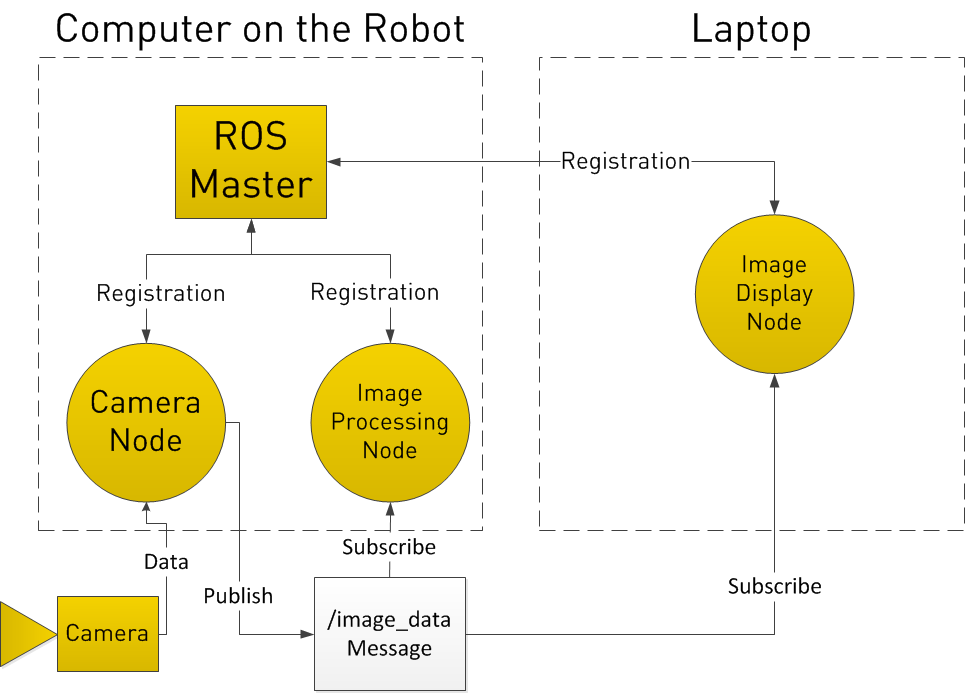
\includegraphics[width=\textwidth]{Bilder/ros_structure.png}
    \caption{ROS Struktur \cite{clearpath_robotics_intro_2015}}
    \label{fig:ros_structure}
\end{figure}

\refFig{fig:ros_structure} zeigt eine mögliche \ac{ROS} Netzwerkstruktur mit Integration einer Kamera und mehreren Computern.

\subsubsection{Entwicklung und Dokumentation}

Da \ac{ROS} von der Community entwickelt wird, sind Ressourcen zum Austausch von Code und Wissen notwendig. Folgendes ist für die Entwicklung besonders relevant:

\begin{description}
    \item[Distributionen] \ac{ROS} ist ähnlich wie Linux-basierte Betriebssysteme in \textit{Distributionen} aufgeteilt. Diese Gliederung sorgt dafür, dass Pakete pro \textit{Distribution} eine bestimmte Softwareversion nutzen \cite[Absatz~3]{romero_rosconcepts_2014}. Dadurch kann eine hohe Kompatibilität zwischen mehreren Paketen gewährleistet werden. Details zu verfügbaren \ac{ROS}-Versionen werden in \refSec{sec:Versionen_ROS} erläutert.
    \item[\ac{ROS} Wiki] Das \textit{\ac{ROS} Community Wiki} ist die Hauptinformationsquelle für Dokumentationen, Tutorials und Korrekturvorschläge \cite[Absatz~3]{romero_rosconcepts_2014}. Einträge können von Jedem nach Erstellen eines Accounts hinzugefügt oder bearbeitet werden. Das \textit{Community Wiki} sollte von Programmierern und Paketerstellern zur Dokumentation genutzt werden.
    \item[Support] Für Neuigkeiten über \ac{ROS} kann das \ac{ROS}-Forum genutzt werden \cite[Absatz~2]{staples_support_2020}. Bei Fehlern, Vorschlägen oder Feature Requests stehen entsprechende Ressourcen zur Eigenrecherche oder Kommunikation zur Verfügung. Aktuelle Links und Leitlinien sind unter \textit{wiki.ros.org/Support} verfügbar \cite[Absatz~3-6]{staples_support_2020}.
\end{description}

\subsection{ROS Versionen} \label{sec:Versionen_ROS}

Wie im letzten Abschnitt erwähnt, gibt es mehrere \ac{ROS}-\textit{Distributionen}. Dabei handelt es sich um Zusammenstellungen von \textit{Packages} miteinander kompatibler Versionen, weshalb sich die Weiterentwicklung der Hauptpakete einer \textit{Distribution} großteils auf Fehlerbehebungen und das Schließen von Sicherheitslücken beschränkt \cite[Absatz~2]{miura_distributions_2021}. Dieses Konzept vereinfacht durch die konstante Code-Basis einer \textit{Distribution} die Entwicklung und Wartung von Softwarepaketen.

Das \textit{Community Wiki} führt Linux als Beispiel für das Konzept der \textit{Distributionen} auf \cite[Absatz~2]{miura_distributions_2021}. Im \ac{ROS}-Kontext sind diese jedoch, besonders bei Betrachtung neuer Versionen, eher mit \textit{Releases} einer einzelnen Linux-Distribution vergleichbar. Frühere \ac{ROS}-Versionen wurden je nach verfügbaren Ressourcen und Nachfrage unterschiedlich lange unterstützt, während aktuelle Releases einen \textit{\ac{LTS}} mit Unterstützungsdauer von fünf Jahren anstreben \cite[Absatz~5]{miura_distributions_2021}. Beim Vergleich zwischen den Daten der Veröffentlichung und Unterstützungsdauer von \ac{ROS} mit den Daten von \textit{Ubuntu LTS} \cite{murray_releases_2021} fallen Parallelen auf. Das Timing der Veröffentlichung neuer \ac{ROS}-Versionen orientiert sich an dem der \textit{Ubuntu LTS}-Versionen.

Da die Aktualisierung der alten Code-Basis von \ac{ROS}-I nicht ohne große Änderungen der Funktionsweise realisierbar ist, wurde 2018 die erste stabile Version von \ac{ROS}-II veröffentlicht. \ac{ROS}-II folgt einem ähnlichen Release-Modell wie die erste Version, wobei die Unterstützungsdauer der jeweiligen Versionen mit ein bis drei Jahren deutlich kürzer ausfällt. Neben den einzelnen Releases gibt es die ,,Rolling Distribution'', die als Version für Entwickler dient und kontinuierlich - auch mit Änderungen, die zu Fehlern im Code führen können - aktualisiert wird \cite{open_robotics_distributions_2021}.

\section{Arten von 3D-Kameras} \ver
Die heutige Arbeit wird in vielen Bereichen durch mobile Roboter sowie stationäre Roboterarme ersetzt. Hierbei spielen vor allem die Genauigkeit sowie die Effizienz eine große Rolle. Die Produktion von Bauteilen, Sortierung, Kartierung und vielen weiteren Arbeitsschritten wurde hauptsächlich durch Kamerasysteme ermöglicht. Diese sind die Augen des Roboters, mit denen der Prozess automatisiert werden kann. Solche Systeme ermöglichen ein autonomes Arbeiten des Roboters und erfordern dadurch zum Beispiel bei einer Qualitätsprüfung, einer Bauteilidentifizierung oder beim Scannen von Produkt-Codes keine Fachkräfte.
Aufgaben, die eine sich ändernde Arbeitsumgebung haben, erfordern eine präzise Umgebungswahrnehmung. Mithilfe einer Kamera kann das Robotersystem so auf veränderte Situationen reagieren. Dadurch steigt zum einen die Flexibilität in Bezug auf die Einsatzbereiche, zum anderen kann durch die Umgebungswahrnehmung so die Wahrscheinlichkeit einer Kollision stark reduziert werden. Beim Einsatz von Kamerasystemen kann man zwischen zwei bekannten Verfahren unterscheiden. Diese werden im folgenden in Bezug auf die Funktion und Einsetzbarkeit verglichen.

\subsection{Stereokamera}\label{sec:Stereokamera} \ver
Die Stereoskopie beschreibt ein Verfahren, welches mithilfe von zweidimensionalen Bildern einen räumlichen Eindruck der Tiefe vermittelt. Eine Stereokamera ist mit zwei nebeneinander angeordneten Kameralinsen ausgestattet. Diese haben einen konstanten Versatz zueinander. Die Verschlüsse der Linsen sind miteinander gekoppelt und müssen nicht individuell eingestellt werden.

Die Funktionsweise der Stereoskopie basiert auf dem binokularen Sehen. Der Ursprung liegt nach Sir David Brewster beim Menschen, indem er das vor ihm liegende Bild durch zwei Augen erkennt und durch die Kombination beider Perspektiven die Tiefen der 2D-Bilder wahrnimmt \cite{sir_david_brewster_stereoscope_1856}. So nimmt die Kamera zwei Bilder aus den jeweiligen Perspektiven der Linsen auf und berechnet mithilfe von Prozessoren und dem mathematischen Verfahren der Triangulierung die Tiefe des zusammengeführten Bildes \cite{waack_stereofotografie_1979}. Dabei muss man jedoch bedenken, dass dieses Verfahren eine hohe Rechenleistung erfordert.

\subsection{RGB-D Kamera}\label{sec:RGB-D_Kamera} \ver
Der Begriff RGB-D beschreibt die Kombination aus einer Farb- und Distanzerkennung. Dabei werden zusätzlich zum einfachen 2D-Farbbild über entsprechende Infrarot-Sensoren die Tiefen gemessen, sodass eine 3D-Aufnahme berechnet werden kann. Dafür wird in der Regel das \ac{ToF} Prinzip genutzt \cite{prof_dr-ing_gunter_pomaska_tiefenkameras_2013}. Dieses sogenannte Laufzeitverfahren misst die Distanzen für jeden Bildpunkt der Szene, indem ein Infrarot-Sensor eine \textit{Point Cloud} auf die Oberfläche projiziert. Die Reflexionen werden von einem CMOS-Bildsensor erkannt. Mit Algorithmen wird die Laufzeit jedes Bildpunktes analysiert und zu Informationen zur Tiefe verarbeitet. Die RGB-Kamera charakterisiert das Bild zusätzlich, um weitere Merkmale festzustellen \cite{prof_dr-ing_gunter_pomaska_tiefenkameras_2013}.

Dadurch, dass die 3D-Aufnahme zusätzlich mit Farbinformationen versehen ist, lassen sich gesamte Szenen und Objekte wesentlich genauer unterscheiden. Bei einer quasi identischen Form können zwei Objekte mit der Farbinformation trotzdem unterschieden werden. Außerdem sind die Anforderungen an Licht- und Umgebungsverhältnisse im Vergleich zur Stereokamera geringer, da die Tiefe mit Infrarot Licht gemessen und nicht berechnet wird. Dennoch sollte genügend Licht für eine saubere Erkennung vorhanden sein. Zudem darf das Sichtfeld der Kamera nicht eingeschränkt werden, damit die Objekte komplett sichtbar sind.

\begin{figure}[ht]
    \centering
    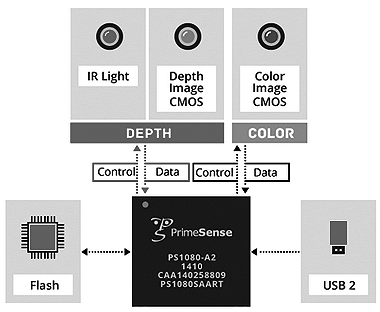
\includegraphics[width=10cm]{Bilder/primeSensor.png}
    \caption{Aufbau RGB-D Kamera \cite{prof_dr-ing_gunter_pomaska_primesensorpng_2013}}
\end{figure}

\section{Objekterkennungsalgorithmen}

Für die Erkennung und Identifikation von Objekten wird ein geeigneter Bild\-erkennungsalgorithmus benötigt. Hauptunterschiede bezüglich der Anwendung sind Genauigkeit, Geschwindigkeit und Hardwareanforderungen im Hinblick auf Leistung. 

Der Algorithmus muss unter den Umgebungsbedingungen des Bauraums zuverlässig funktionieren und ausreichend schnell sein, um keine großen Verzögerungen durch die Erkennung zu verursachen. Die Schnittstelle zu \ac{ROS} muss außerdem die Möglichkeit bieten, Positionsdaten der Objekte an das System weiterzugeben, um die Lokalisierung dieser zu ermöglichen. Die Weitergabe der Tiefenkoordinate durch das Objekterkennungsprogramm ist hierbei optional, da diese auch durch Abgleich der 2D-Koordinaten mit dem Tiefensensor berechnet werden kann. Da in der Arbeit mehrere Objekte verwendet werden, ist zudem die Unterstützung zur Erkennung verschiedener Bauteile im gleichen Bild notwendig.

Die Ansätze von Objekterkennungsalgorithmen können in traditionelle und moderne Ansätze gegliedert werden. Letztere basieren auf \textit{\ac{DL}} und sind grundsätzlich für ein breiteres Spektrum an Objekten geeignet \cite[Absatz~2]{mohan_6_2020}. Folgend werden die Ansätze verglichen und Algorithmen aufgeführt, die gut in \ac{ROS} integrierbar sind und mit RGB-Kamerasystemen funktionieren.

\subsection{Traditionelle Computer Vision}

\textit{\ac{SIFT}} von Lowe \cite{lowe_distinctive_2004} und \textit{\ac{SURF}} von Bay et al. \cite{bay_surf_2006} sind Algorithmen, die auf \textit{Keypoints} in Bildern basieren, welche vom jeweiligen Algorithmus generiert und zur Erkennung von Objekten bei einer bestimmten Übereinstimmungsrate genutzt werden können. \textit{Keypoints} sind um Punkte im Bild, die nahezu invariant gegenüber der Bildparameter wie Vergrößerung, Verzerrung und Rotation sind und somit gut als Orientierungspunkte genutzt werden können \cite[Kapitel~13]{lowe_distinctive_2004}.

Genannte Techniken können für traditionelle Ansätze genutzt werden. Diese funktionieren grundsätzlich folgendermaßen: Zuerst wird die Position der Objekte im Bild durch Scannen des kompletten Bildes näherungsweise bestimmt. Anschließend können Techniken wie beispielsweise \textit{\ac{SIFT}} genutzt werden, um relevante Merkmale der Objekte zu extrahieren. Zuletzt werden Algorithmen wie \textit{\ac{SVM}} \cite{cortes_support-vector_1995} zur Identifikation der Objektkategorie genutzt \cite[Kapitel~1]{youzi_review_2020}. \refFig{fig:detection_traditional} zeigt den beschriebenen Ablauf.

\begin{figure}[ht]
    \centering
    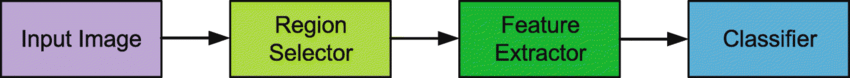
\includegraphics[width=\textwidth]{Bilder/detection_traditional.png}
    \caption{Traditioneller Ansatz \cite[Abbildung~3]{youzi_review_2020}}
    \label{fig:detection_traditional}
\end{figure}

Traditionelle \textit{\ac{CV}} kann durch die geringere Komplexität effizienter als \textit{\ac{DL}} sein. Auch bei Abweichung der zu erkennenden Objekte vom Datensatz, der zum Training des Algorithmus genutzt wird, sind Algorithmen der traditionellen \textit{\ac{CV}} manchmal besser geeignet. Im Gegensatz zu \textit{\ac{DL}} ist traditionelle \textit{\ac{CV}} mit hohem Forschungsaufwand beim Einlernprozess verbunden. \cite[Absatz~2.3]{arai_deep_2020}.

Eine Möglichkeit zur Integration traditioneller Bilderkennung in \ac{ROS} bietet beispielsweise das Paket \textit{find\_object\_2d}, das neben Objektklassifikation und Positionserkennung auch die dreidimensionale Orientierung von Objekten im Raum erkennen kann \cite{labbe_find_2011}.

Aufgrund des Forschungsaufwandes zum Einlernen der Objekte und der hohen Abhängigkeit von der Art und Form zu erkennender Teile eignet sich diese Art der Bilderkennung nur mäßig für den vorliegenden Fall.

\subsection{Deep Learning}

Verglichen mit traditioneller Bilderkennung werden beim \textit{\ac{DL}} keine mathematischen Modelle durch manuelles Sammeln und Auswerten von Prozessdaten (Deskriptive Analytik) oder Erstellen eines prädiktiven Modells (Prädiktive Analytik) erstellt \cite[Kapitel~1]{bonaccorso_machine_2018}. Stattdessen werden \textit{Neural Networks} verwendet. Diese sind mit dem menschlichen Gehirn vergleichbar, da sie aus vielen interagierenden Berechnungszellen bestehen, die zur Entscheidungsfindung miteinander kommunizieren \cite[Kapitel~3~Abschnitt~B]{o_mahony_adaptive_2016}. Dabei fällt der Schritt der Feature-Extraktion weg. Man unterscheidet zwischen \textit{\acp{ANN}}, \textit{\acp{CNN}} und \textit{\acp{RNN}}. Im Rahmen dieser Arbeit wird verstärkt auf die aktuell weit verbreiteten \textit{\acp{CNN}} eingegangen, da diese für viele Anwendungsfälle den besten Kompromiss zwischen Genauigkeit und Geschwindigkeit darstellen.

State of The Art Methoden zur Objekterkennung basieren auf \textit{\acp{DCNN}}. Dabei kann laut Yurtsever et al. zwischen ,,Single Stage Detection Frameworks'', die die Position und Klassifikation simultan durchführen und ,,Region Proposal Detection Frameworks'' unterscheiden werden, bei denen die Kategorisierung in einem zusätzlichen Schritt erfolgt \cite[Kapitel~V,~Absatz~A]{yurtsever_survey_2020}.

Aktuell sind \acp{DCNN} - besonders Single-Stage-Algorithmen - aufgrund der hohen Erkennungsrate in kurzer Zeit besonders relevant. Aufgrund der weiten Verbreitung und somit aktiven Weiterentwicklung, dem vergleichsweise einfachen Prozess zum Einlernen neuer Objekte und einem für das Projekt geeigneten Kompromiss zwischen Geschwindigkeit und Genauigkeit wird hier der Fokus auf den \textit{\ac{YOLO}}-Algorithmus gelegt.

Beim ursprünglich von Redmon et al. entwickelten \textit{\ac{YOLO}}-Algorithmus \cite{redmon_you_2016} handelt es sich um einen \textit{Single-Stage Detector}. Anders als bei \textit{Two-Stage} Algorithmen werden nicht erst Bildabschnitte, die Objekte enthalten könnten, vorgeschlagen. Stattdessen findet die Objekterkennung, -klassifikation und Wahrscheinlichkeitsvorhersage in einem Schritt statt \cite{bandyopadhyay_yolo_2021}. Der Algorithmus teilt Bilder in Regionen auf und erkennt und lokalisiert Objekte in allen Teilen gleichzeitig. Dabei werden sogenannte ,,Bounding Boxes'', die sich mit den Eckpunkten der Objekte decken, generiert \cite[Absatz~2.1.3]{zou_object_2019}.

\begin{figure}[ht]
    \centering
    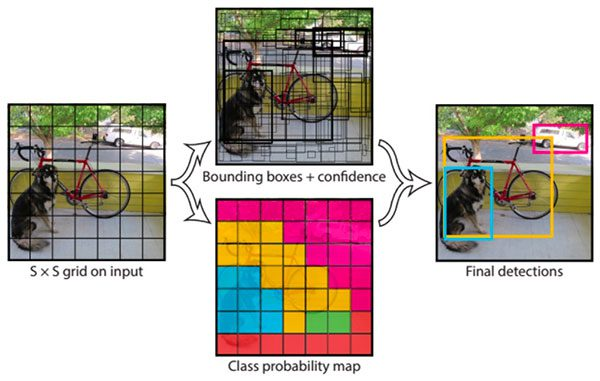
\includegraphics[width=\textwidth]{Bilder/detection_yolo.jpg}
    \caption{Vereinfachte Struktur von YOLO \cite{redmon_you_2016}}
    \label{fig:detection_yolo}
\end{figure}

\refFig{fig:detection_yolo} zeigt die Zerlegung zur Generierung von \textit{Bounding Boxes}. In allen Teilen des Rasters wird eine Objekterkennung und -lokalisierung durchgeführt, auf die die Generierung von \textit{Bounding Boxes} mit Koordinaten relativ zum jeweiligen Teil folgt. Duplikate, die durch über mehrere Teile reichende Objekte entstehen, werden in einem mehrstufigen Prozess mithilfe von \textit{Non-Maximum Suppression} zusammengefasst. \cite[Abschnitt~4]{bandyopadhyay_yolo_2021}

\pagebreak
Ein \textit{\ac{DCNN}} wird hier genutzt, um Bildmerkmale zu extrahieren, was zu einer Verringerung der Auflösung und somit geringeren Ressourcenanforderungen führt \cite[Kapitel~V,~Absatz~A]{yurtsever_survey_2020}. Eine Implementierung des Algorithmus wurde von Redmon selbst unter dem Namen ,,Darknet'' veröffentlicht \cite{redmon_darknet_2021}. Nach der Ankündigung von Redmon, den Algorithmus aufgrund ethischer Bedenken nicht weiterzuentwickeln \cite{joseph_redmon_i_2020}, wurde 2020 eine weitere auf \textit{Darknet} basierende Version von Bochkovskiy et al. veröffentlicht \cite{bochkovskiy_yolov4_2020}.

Im Rahmen dieser Arbeit wird die Version \textit{YOLOv3 Tiny} genutzt. Dabei handelt es sich um eine Version, die speziell auf schwache Hardware ausgelegt ist und somit im Anwendungsfall mit einer hohen Bildwiederholrate betrieben werden kann. Diese ist zur Ermittlung des Objektmittelpunktes bei der Annäherung an die Bauteile vorteilhaft. Die Integration des \textit{Darknet} Frameworks in \ac{ROS} erfolgt mit dem Paket \textit{darknet\_ros} \cite{bjelonic_yolo_2016}.